%%%%%%%%%%%%%%%%%%%%%%%%%%%%%%%%%%%%%%%%%%%%%%%%%%%%%%%%%%%%%%%%%%%%%%%%%%%%%%%%
%2345678901234567890123456789012345678901234567890123456789012345678901234567890
%        1         2         3         4         5         6         7         8

%\documentclass[letterpaper, 10 pt, conference]{ieeeconf}  % Comment this line out
                                                           % if you need a4paper
\documentclass[a4paper, 10pt, conference]{ieeeconf}        % Use this line for a4
                                                           % paper

%\IEEEoverridecommandlockouts                              % This command is only
                                                          % needed if you want to
                                                          % use the \thanks command
%\overrideIEEEmargins
% See the \addtolength command later in the file to balance the column lengths
% on the last page of the document



% The following packages can be found on http:\\www.ctan.org
\usepackage{graphicx} % for pdf, bitmapped graphics files
%\usepackage{caption}
%\usepackage{subfigure}
\usepackage{subcaption}
\usepackage{epsfig} % for postscript graphics files
\usepackage{mathptmx} % assumes new font selection scheme installed
\usepackage{times} % assumes new font selection scheme installed
\usepackage{amsmath} % assumes amsmath package installed
\usepackage{amssymb}  % assumes amsmath package installed
\usepackage{enumerate}
\usepackage{mcode} %  [framed]
\usepackage{url}
\usepackage[bookmarks]{hyperref}
\usepackage{setspace}
\usepackage{paralist}
\begin{document}
\title{\LARGE \bf
Image segmentation
}

\author{ \parbox{3 in}{\centering Daniel Barmaimon \\
%         \thanks{*Use the $\backslash$thanks command to put information here}\\
         \ Medical Image Analysis - Vibot Master\\
         \ University of Girona\\         
}}

\maketitle
%\thispagestyle{empty}
%\pagestyle{empty}

\graphicspath{{./images/}}






%%%%%%%%%%%%%%%%%%%%%%%%%%%%%%%%%%%%%%%%%%%%%%%%%%%%%%%%%%%%%%%%%%%%%%%%%%%%%%%%
\begin{abstract}

The main purpose of this lab is to understand the different kind of method used in segmentation for medical image analysis and the pros and cons of the choice made.
\end{abstract}


%%%%%%%%%%%%%%%%%%%%%%%%%%%%%%%%%%%%%%%%%%%%%%%%%%%%%%%%%%%%%%%%%%%%%%%%%%%%%%%%
\section{Introduction}
A correct segmentation is basic to let the experts analyze the image without missing detail or adding any non-expected element. During this lab three main tasks will be implemented. First one is to get a single ground true taken from the handmade binary mask of three different experts. Second one will be to study the differences of using several method to get the segmentation and how good they were. Last one will be related with the implementation of a method by my own.

\section{Ground-truth generation}
To get a the ground-truth of the images, three different binary mask created by three different experts will be used. The implementation used will give any pixel as positive, if at least two of the three doctors coincide in its value, and it will be given a negative value otherwise.\\
The implementation used considered the use of binary operations to get the final ground truth image, avoiding the use of a loop to get the vote for each pixel.
\begin{lstlisting}
clear all
clc
tic;
%% Read the images
dataFilePathGT1 = ...
fullfile(pwd,'images','gt','expert_1');
dataFilePathGT2 = ...
fullfile(pwd,'images','gt','expert_2');
dataFilePathGT3 = ...
fullfile(pwd,'images','gt','expert_3');

dataFilePathOriginal = ...
fullfile(pwd,'images','original');

fileNamesGT1 = dir(fullfile(dataFilePathGT1,'*.png'));
fileNamesGT2 = dir(fullfile(dataFilePathGT2,'*.png'));
fileNamesGT3 = dir(fullfile(dataFilePathGT3,'*.png'));

% get number of images
N = numel(fileNamesGT1);
height = 387;                 
width = 632;
% read all images
data = zeros(height, width, 3*N);
for i=1:N    
    img = ...
    imread(fullfile...
    (dataFilePathGT1,fileNamesGT1(i).name));
    data(:,:,i) = img;
end
for i=1:N 
    img = ...
    imread(fullfile...
    (dataFilePathGT2,fileNamesGT2(i).name));
    data(:,:,i+N) = img;
end
for i=1:N 
    img = ...
    imread(fullfile...
    (dataFilePathGT3,fileNamesGT3(i).name));
    data(:,:,i+2*N) = img;
end
%% Weight the images and fusion the masks
fusion = zeros(height, width, N);
for i=1:N
    fusion(:,:,i)=...
    (data(:,:,i).*data(:,:,i+N)) +...
    (data(:,:,i).*data(:,:,i+2*N)) +...
    (data(:,:,i+N).*data(:,:,i+2*N));
    A = fusion(:,:,i);
    figure;
    imshow(A);
end
time = toc
\end{lstlisting}


The time obtained after processing the unique ground true with this algorithm, for 8 different images, was 0.4069 s. without showing the images, and 1.7686 s. if the images are shown. In the next page, the original images, the ground truth images (made by each expert) and the fusion of these images will be shown.
\clearpage
\begin{figure}[ht!]
 \centering
 \begin{tabular}{c c c c c}
 \begin{subfigure}{0.2\textwidth}
 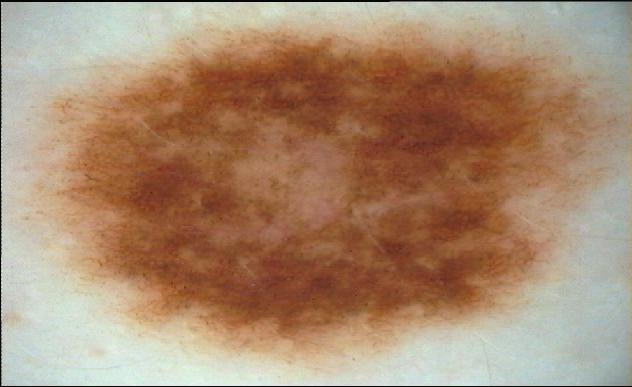
\includegraphics[scale=0.15]{original01.JPG}
 \end{subfigure}
 \begin{subfigure}{0.2\textwidth}
 
\includegraphics[scale=0.2]{expert_1GroundTrue_01.JPG}
 \end{subfigure}
 \begin{subfigure}{0.2\textwidth}
  
\includegraphics[scale=0.2]{expert_2GroundTrue_01.JPG}
  \end{subfigure} 
 \begin{subfigure}{0.2\textwidth}
  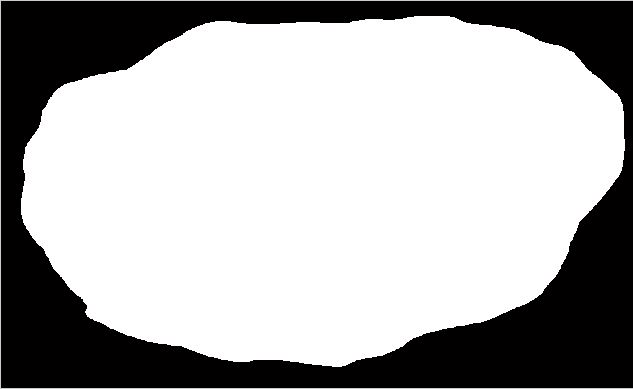
\includegraphics[scale=0.2]{expert_3GroundTrue_01.JPG}
  \end{subfigure} 
 \begin{subfigure}{0.2\textwidth}
  
\includegraphics[scale=0.2]{finalGroundTrue_01.JPG}
  \end{subfigure} \\ \\
   \begin{subfigure}{0.2\textwidth}
   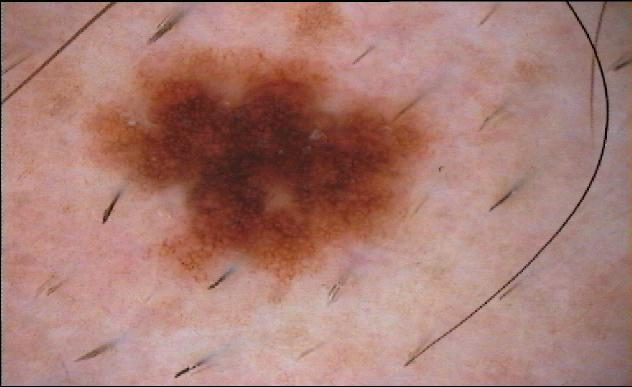
\includegraphics[scale=0.15]{original02.JPG}
   \end{subfigure}
   \begin{subfigure}{0.2\textwidth}
   
\includegraphics[scale=0.2]{expert_1GroundTrue_02.JPG}
   \end{subfigure}
   \begin{subfigure}{0.2\textwidth}
    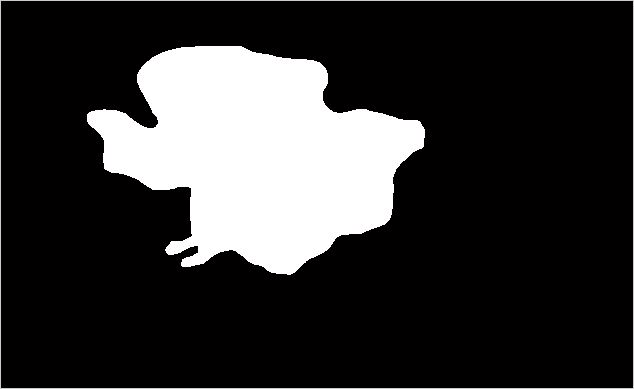
\includegraphics[scale=0.2]{expert_2GroundTrue_02.JPG}
    \end{subfigure} 
   \begin{subfigure}{0.2\textwidth}
    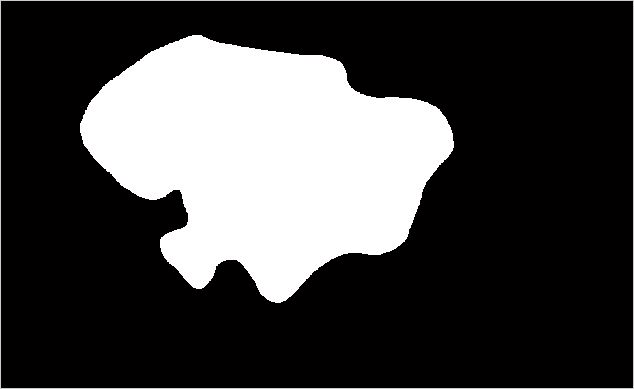
\includegraphics[scale=0.2]{expert_3GroundTrue_02.JPG}
    \end{subfigure} 
   \begin{subfigure}{0.2\textwidth}
    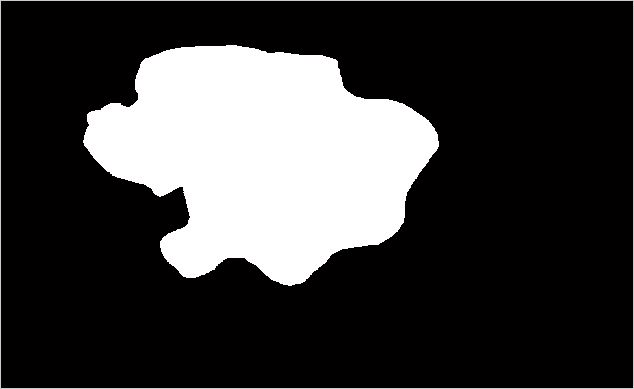
\includegraphics[scale=0.2]{finalGroundTrue_02.JPG}
    \end{subfigure} \\ \\
     \begin{subfigure}{0.2\textwidth}
     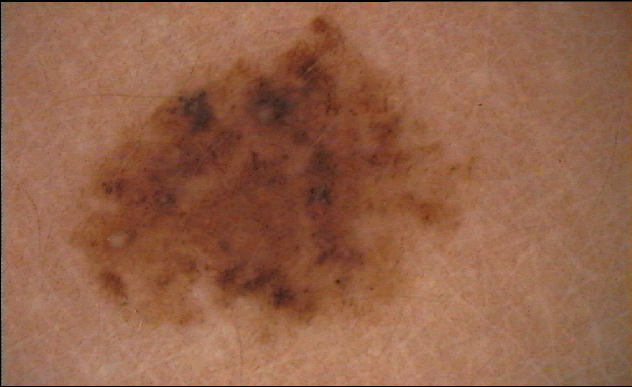
\includegraphics[scale=0.15]{original03.JPG}
     \end{subfigure}
     \begin{subfigure}{0.2\textwidth}
     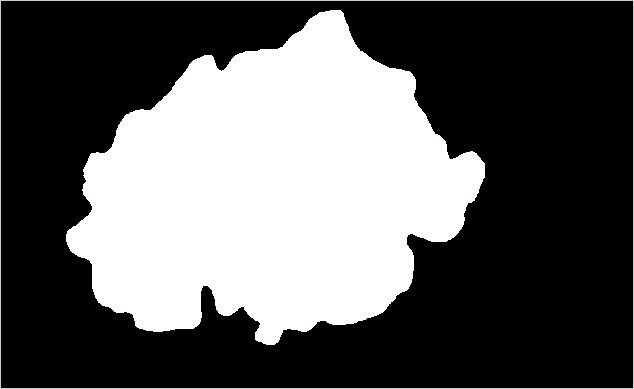
\includegraphics[scale=0.2]{expert_1GroundTrue_03.JPG}
     \end{subfigure}
     \begin{subfigure}{0.2\textwidth}
      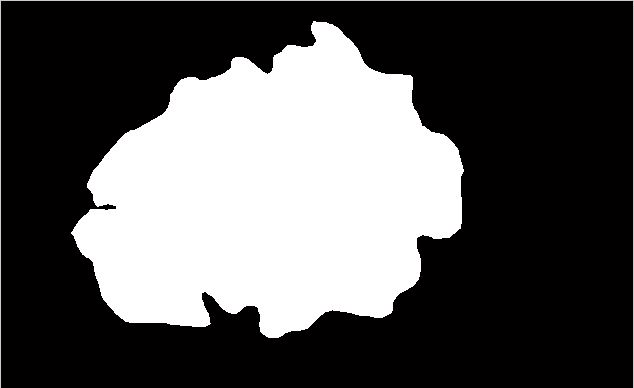
\includegraphics[scale=0.2]{expert_2GroundTrue_03.JPG}
      \end{subfigure} 
     \begin{subfigure}{0.2\textwidth}
      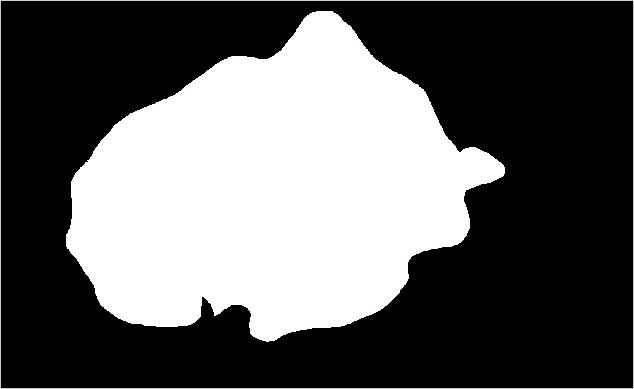
\includegraphics[scale=0.2]{expert_3GroundTrue_03.JPG}
      \end{subfigure} 
     \begin{subfigure}{0.2\textwidth}
      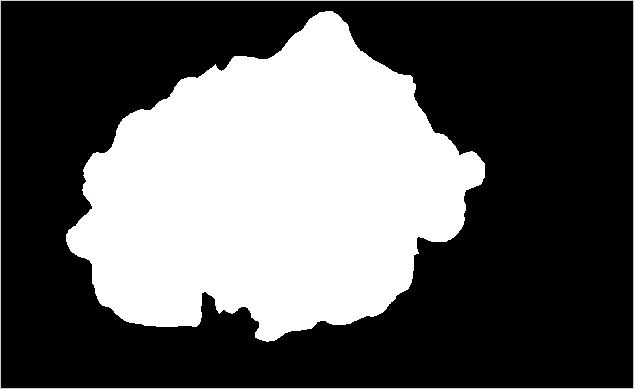
\includegraphics[scale=0.2]{finalGroundTrue_03.JPG}
      \end{subfigure} \\ \\
       \begin{subfigure}{0.2\textwidth}
       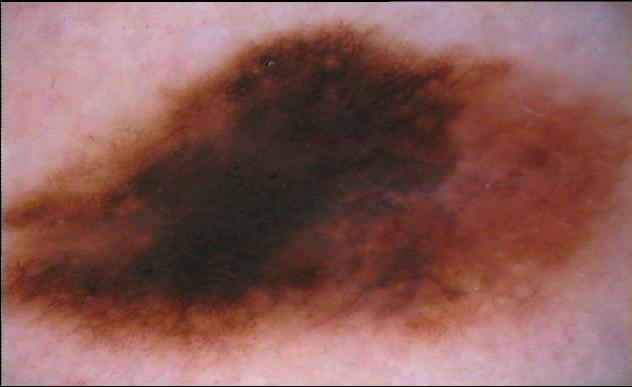
\includegraphics[scale=0.15]{original04.JPG}
       \end{subfigure}
       \begin{subfigure}{0.2\textwidth}
       
\includegraphics[scale=0.2]{expert_1GroundTrue_04.JPG}
       \end{subfigure}
       \begin{subfigure}{0.2\textwidth}
        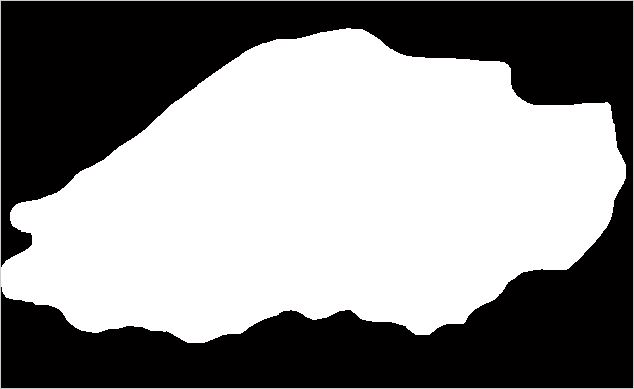
\includegraphics[scale=0.2]{expert_2GroundTrue_04.JPG}
        \end{subfigure} 
       \begin{subfigure}{0.2\textwidth}
        
\includegraphics[scale=0.2]{expert_3GroundTrue_04.JPG}
        \end{subfigure} 
       \begin{subfigure}{0.2\textwidth}
        
\includegraphics[scale=0.2]{finalGroundTrue_04.JPG}
        \end{subfigure} \\ \\
         \begin{subfigure}{0.2\textwidth}
         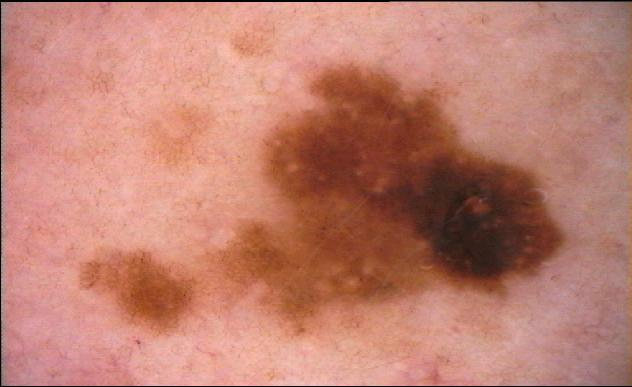
\includegraphics[scale=0.15]{original05.JPG}
         \end{subfigure}
         \begin{subfigure}{0.2\textwidth}
         
\includegraphics[scale=0.2]{expert_1GroundTrue_05.JPG}
         \end{subfigure}
         \begin{subfigure}{0.2\textwidth}
          
\includegraphics[scale=0.2]{expert_2GroundTrue_05.JPG}
          \end{subfigure} 
         \begin{subfigure}{0.2\textwidth}
          
\includegraphics[scale=0.2]{expert_3GroundTrue_05.JPG}
          \end{subfigure} 
         \begin{subfigure}{0.2\textwidth}
          
\includegraphics[scale=0.2]{finalGroundTrue_05.JPG}
          \end{subfigure} \\ \\
   \begin{subfigure}{0.2\textwidth}
   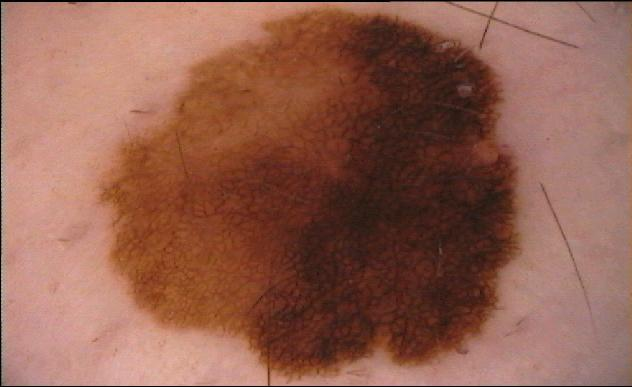
\includegraphics[scale=0.15]{original06.JPG}
   \end{subfigure}
   \begin{subfigure}{0.2\textwidth}
   
\includegraphics[scale=0.2]{expert_1GroundTrue_06.JPG}
   \end{subfigure}
   \begin{subfigure}{0.2\textwidth}
    
\includegraphics[scale=0.2]{expert_2GroundTrue_06.JPG}
    \end{subfigure} 
   \begin{subfigure}{0.2\textwidth}
    
\includegraphics[scale=0.2]{expert_3GroundTrue_06.JPG}
    \end{subfigure} 
   \begin{subfigure}{0.2\textwidth}
    
\includegraphics[scale=0.2]{finalGroundTrue_06.JPG}
    \end{subfigure} \\ \\
     \begin{subfigure}{0.2\textwidth}
     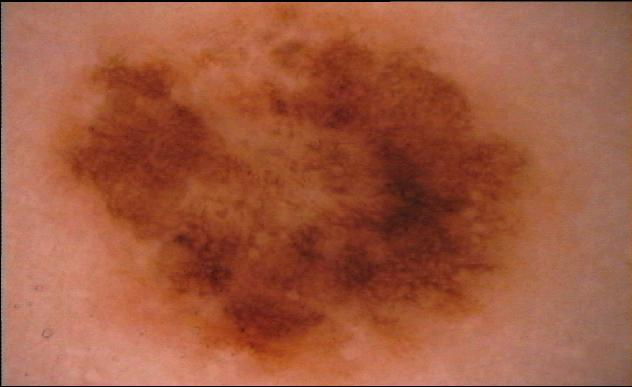
\includegraphics[scale=0.15]{original07.JPG}
     \end{subfigure}
     \begin{subfigure}{0.2\textwidth}
     
\includegraphics[scale=0.2]{expert_1GroundTrue_07.JPG}
     \end{subfigure}
     \begin{subfigure}{0.2\textwidth}
      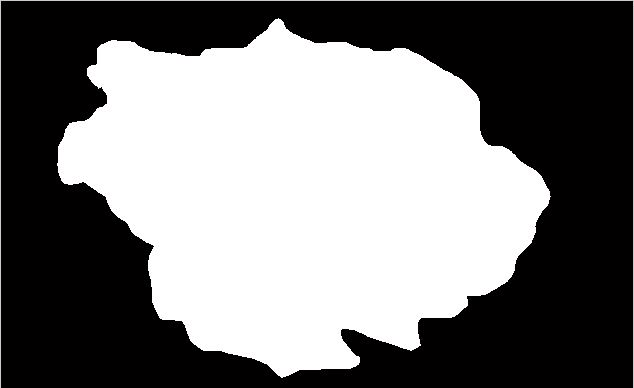
\includegraphics[scale=0.2]{expert_2GroundTrue_07.JPG}
      \end{subfigure} 
     \begin{subfigure}{0.2\textwidth}
      
\includegraphics[scale=0.2]{expert_3GroundTrue_07.JPG}
      \end{subfigure} 
     \begin{subfigure}{0.2\textwidth}
      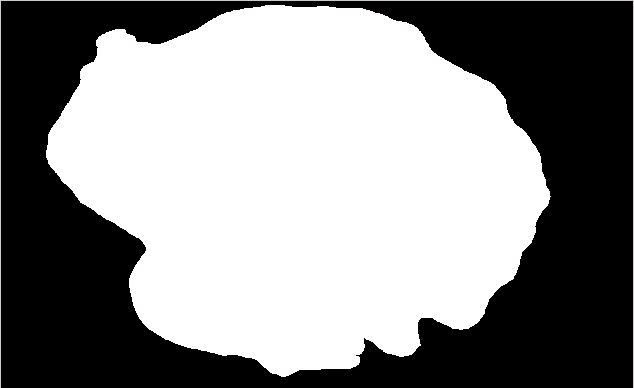
\includegraphics[scale=0.2]{finalGroundTrue_07.JPG}
      \end{subfigure} \\ \\
       \begin{subfigure}{0.2\textwidth}
       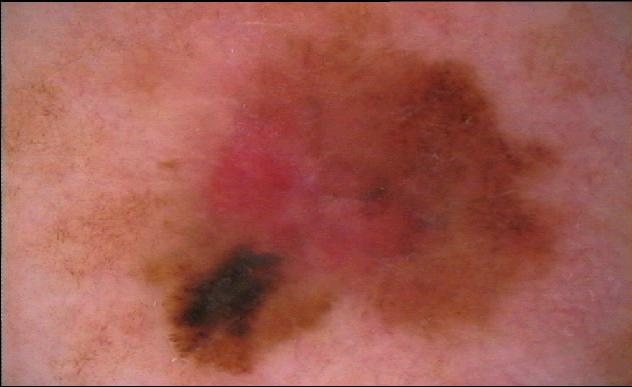
\includegraphics[scale=0.15]{original08.JPG}
       \end{subfigure}
       \begin{subfigure}{0.2\textwidth}
       
\includegraphics[scale=0.2]{expert_1GroundTrue_08.JPG}
       \end{subfigure}
       \begin{subfigure}{0.2\textwidth}
        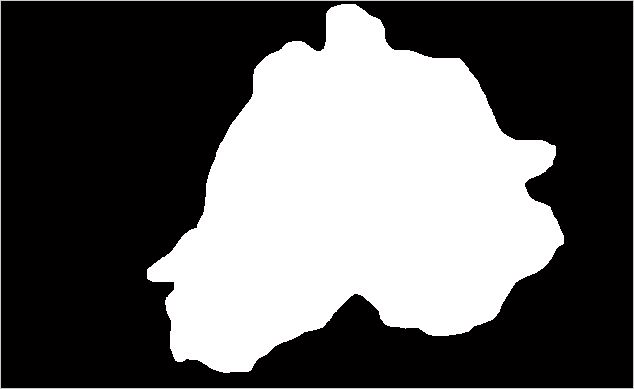
\includegraphics[scale=0.2]{expert_2GroundTrue_08.JPG}
        \end{subfigure} 
       \begin{subfigure}{0.2\textwidth}
        
\includegraphics[scale=0.2]{expert_3GroundTrue_08.JPG}
        \end{subfigure} 
       \begin{subfigure}{0.2\textwidth}
        
\includegraphics[scale=0.2]{finalGroundTrue_08.JPG}
        \end{subfigure} \\
 \end{tabular}

% \caption{Multimodal image fusion and reconstruction of anatomical model} 
\end{figure}    
\clearpage
\section{Segmentation}
In this section three different methods for segmenting these images will be analyzed and compared.
\subsection{PDF-based segmentation}
For this method the first step will be to change from RGB to XYZ, avoiding the problems of negative values for channels R, G and B. Then the image is transformed to gray scale and the borders are removed. This is the initialization step. \\
Next part of the process will be to get a local minimum. For getting this, a histogram is performed. To avoid the discontinuities a line that smooth the histogram will be draw joining the peaks for each beam of the histogram with a smooth line. 
If the local minimum is found before a predefine value (in this case 0.4), it will be used as threshold.\\
\begin{figure}[ht!]
 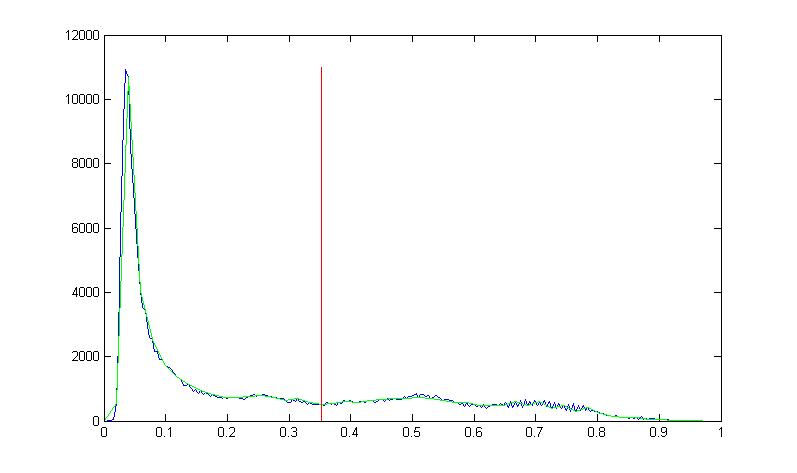
\includegraphics[scale=0.3]{/images/seg/pdfBased/histogram.JPG}\caption{Histogram (b), smoothed histogram (g) and threshold (r)}
\end{figure} \\
Once the threshold is applied to the image the holes are filled and the border replaced.
If there isn't a local minimum, a predefined threshold will be used. 
The result of the mask obtained for each image is shown in next figures.

\begin{figure}[ht!]
 \centering
 \begin{tabular}{c c}
 \begin{subfigure}{0.2\textwidth}
 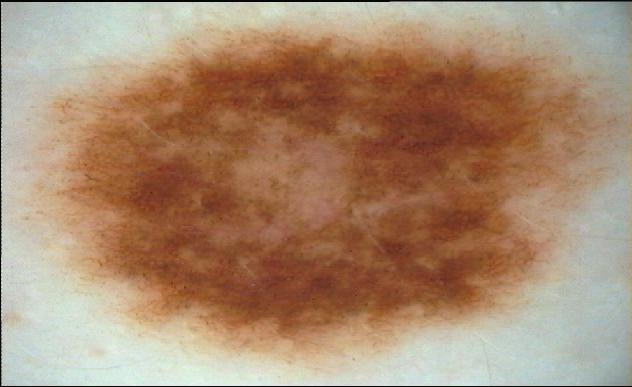
\includegraphics[scale=0.15]{original01.JPG}\caption{}
 \end{subfigure}
 \begin{subfigure}{0.2\textwidth}
 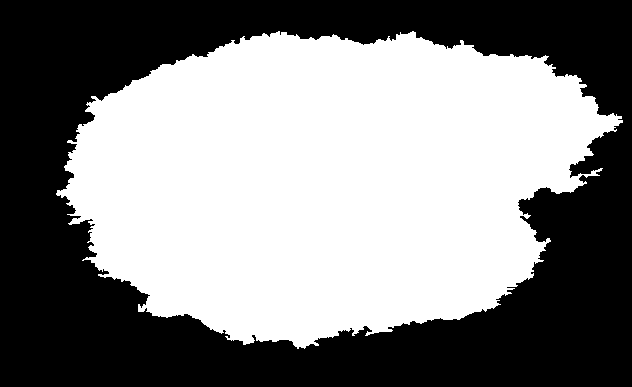
\includegraphics[scale=0.15]{/images/seg/pdfBased/1.png}\caption{}
 \end{subfigure}\\
 \begin{subfigure}{0.2\textwidth}
  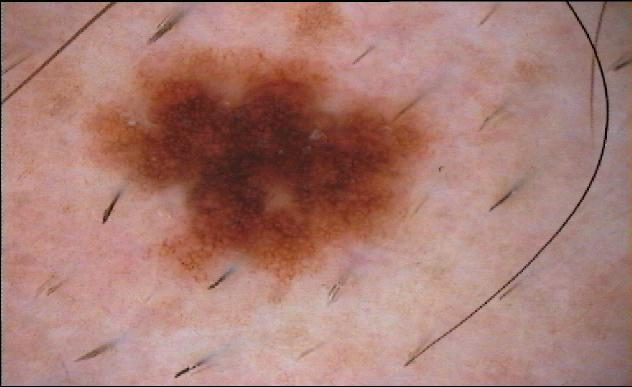
\includegraphics[scale=0.15]{original02.JPG}\caption{}
  \end{subfigure}
  \begin{subfigure}{0.2\textwidth}
  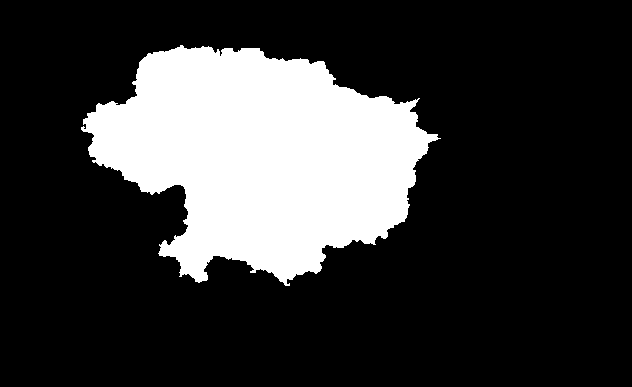
\includegraphics[scale=0.15]{/images/seg/pdfBased/2.png}\caption{}
  \end{subfigure}\\
 \begin{subfigure}{0.2\textwidth}
  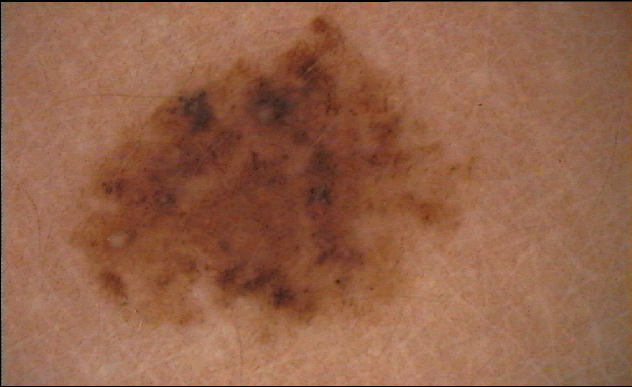
\includegraphics[scale=0.15]{original03.JPG}\caption{}
  \end{subfigure}
  \begin{subfigure}{0.2\textwidth}
  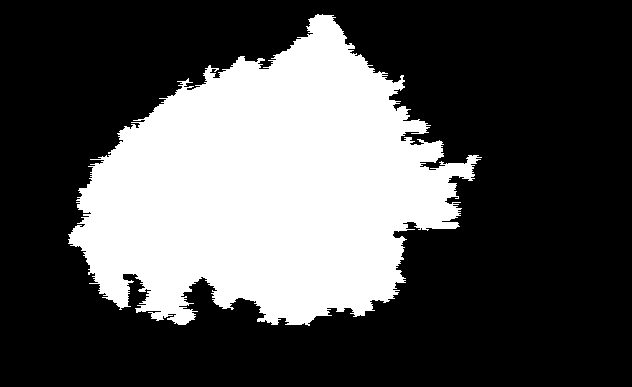
\includegraphics[scale=0.15]{/images/seg/pdfBased/3.png}\caption{}
  \end{subfigure}\\
 \begin{subfigure}{0.2\textwidth}
  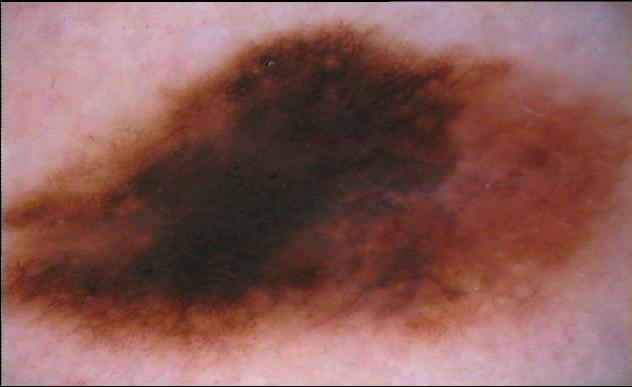
\includegraphics[scale=0.15]{original04.JPG}\caption{}
  \end{subfigure}
  \begin{subfigure}{0.2\textwidth}
  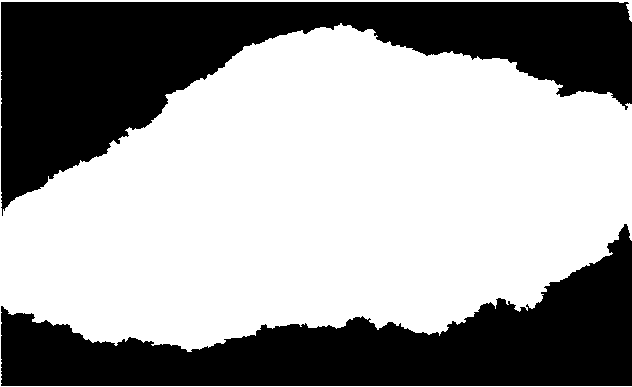
\includegraphics[scale=0.15]{/images/seg/pdfBased/4.png}\caption{}
  \end{subfigure}\\
 \begin{subfigure}{0.2\textwidth}
 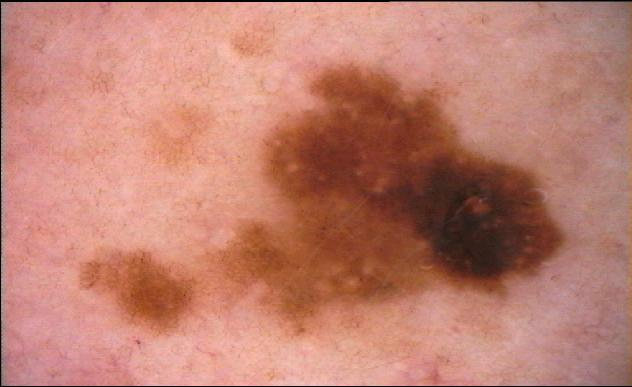
\includegraphics[scale=0.15]{original05.JPG}\caption{}
 \end{subfigure}
 \begin{subfigure}{0.2\textwidth}
 \includegraphics[scale=0.15]{/images/seg/pdfBased/5.png}\caption{}
 \end{subfigure}\\
 \begin{subfigure}{0.2\textwidth}
  \includegraphics[scale=0.15]{original06.JPG}\caption{}
  \end{subfigure}
  \begin{subfigure}{0.2\textwidth}
  \includegraphics[scale=0.15]{/images/seg/pdfBased/6.png}\caption{}
  \end{subfigure}\\
 \begin{subfigure}{0.2\textwidth}
  \includegraphics[scale=0.15]{original07.JPG}\caption{}
  \end{subfigure}
  \begin{subfigure}{0.2\textwidth}
  \includegraphics[scale=0.15]{/images/seg/pdfBased/7.png}\caption{}
  \end{subfigure}\\
 \begin{subfigure}{0.2\textwidth}
  \includegraphics[scale=0.15]{original08.JPG}\caption{}
  \end{subfigure}
  \begin{subfigure}{0.2\textwidth}
  \includegraphics[scale=0.15]{/images/seg/pdfBased/8.png}\caption{}
  \end{subfigure}\\    
 \end{tabular}
 \end{figure}
\clearpage
\subsection{Fuzzy C-Means segmentation}
The method is based in a clustering algorithm that produces an optimal \textit{c} partition by minimizing an object function by iteratively updating membership function and cluster centers. The object function is the weighted sum of distance of data from cluster centers.\\
Any point \textit{x} has a set of coefficients \textit{$ w_{k}(x)$} (as many as number of clusters) and each one of them will measure how likely is the point to belong to each cluster. \\
\begin{equation}
w_{k}(x)=\frac{1}{\sum\limits_{j}(\frac{d(center_{k},x)}{d(center_{j},x)})^{2/(m-1)}}
\end{equation}
The centroid of each cluster is the mean of all points, weighted by the previous coefficients.
\begin{equation}
c_{k}=\dfrac{\sum\limits_{x}w_{k}(x)^mx}{\sum\limits_{x}w_{k}(x)^m}
\end{equation}
The parameter \textit{m} allows to give more or less weight to the distance to each cluster.\\
The algorithm will be compounded by the following steps:
\begin{enumerate}

\item Choose the number of clusters
\item Assign randomly to each point coefficients for being in the clusters.
\item Repeat until the algorithm converges (variation between two steps should be less than  $\varepsilon$)
	\begin{enumerate}[(a)]
		\item Compute the centroid for each cluster, using formula above.
		\item For each point, compute its coefficients of being in the clusters, using the formula above.
	\end{enumerate}
\end{enumerate}
\begin{figure}[ht!]
 \centering
 \begin{tabular}{c c}
 \begin{subfigure}{0.2\textwidth}
 \includegraphics[scale=0.15]{original01.JPG}\caption{}
 \end{subfigure}
 \begin{subfigure}{0.2\textwidth}
 \includegraphics[scale=0.15]{/images/seg/fuzzyCMeans/1.png}\caption{}
 \end{subfigure}\\
 \begin{subfigure}{0.2\textwidth}
  \includegraphics[scale=0.15]{original02.JPG}\caption{}
  \end{subfigure}
  \begin{subfigure}{0.2\textwidth}
  \includegraphics[scale=0.15]{/images/seg/fuzzyCMeans/2.png}\caption{}
  \end{subfigure}\\
 \begin{subfigure}{0.2\textwidth}
  \includegraphics[scale=0.15]{original03.JPG}\caption{}
  \end{subfigure}
  \begin{subfigure}{0.2\textwidth}
  \includegraphics[scale=0.15]{/images/seg/fuzzyCMeans/3.png}\caption{}
  \end{subfigure}\\
 \begin{subfigure}{0.2\textwidth}
  \includegraphics[scale=0.15]{original04.JPG}\caption{}
  \end{subfigure}
  \begin{subfigure}{0.2\textwidth}
  \includegraphics[scale=0.15]{/images/seg/fuzzyCMeans/4.png}\caption{}
  \end{subfigure}\\
 \begin{subfigure}{0.2\textwidth}
 \includegraphics[scale=0.15]{original05.JPG}\caption{}
 \end{subfigure}
 \begin{subfigure}{0.2\textwidth}
 \includegraphics[scale=0.15]{/images/seg/fuzzyCMeans/5.png}\caption{}
 \end{subfigure}\\
 \begin{subfigure}{0.2\textwidth}
  \includegraphics[scale=0.15]{original06.JPG}\caption{}
  \end{subfigure}
  \begin{subfigure}{0.2\textwidth}
  \includegraphics[scale=0.15]{/images/seg/fuzzyCMeans/6.png}\caption{}
  \end{subfigure}\\
 \begin{subfigure}{0.2\textwidth}
  \includegraphics[scale=0.15]{original07.JPG}\caption{}
  \end{subfigure}
  \begin{subfigure}{0.2\textwidth}
  \includegraphics[scale=0.15]{/images/seg/fuzzyCMeans/7.png}\caption{}
  \end{subfigure}\\
 \begin{subfigure}{0.2\textwidth}
  \includegraphics[scale=0.15]{original08.JPG}\caption{}
  \end{subfigure}
  \begin{subfigure}{0.2\textwidth}
  \includegraphics[scale=0.15]{/images/seg/fuzzyCMeans/8.png}\caption{}
  \end{subfigure}\\    
 \end{tabular}
 \end{figure}
 
 \clearpage
 \subsection{Level set segmentation}
 This is an important category for segmentation based on partial differential equations (PDE), i.e. progressive evaluation of the differences among neighboring pixels to find object boundaries. Ideally, the algorithm will converge at the boundary of the object where the differences are the highest. There are several algorithm but the main idea of most of them can be expressed in three simple steps.
 \begin{enumerate}
 \item Initialize/reinitialize $\phi$ at $t = t^{n}$
 \item Construct/approximate $H(t,x,\phi,D\phi,D^{2}\phi)$. 
 \item Evolve
	 \begin{equation}
 		\phi_{t} + H(t,x,\phi,D\phi,D^{2}\phi) = 0
	 \end{equation}
	 for $ t = t_{n} + \Delta t $
 \end{enumerate}
 In the case it is being studied the image Z channel of the image is transform into gray-scale image, and a window (where it is known that the lesion would be) in the middle of the screen is given as initialization parameter. Also last processed image, the number of initial and end iterations, a mask to allow a smoothed result, regularization parameter for normalization of the distances are given as parameters. \\
 As this is an iterative method is the one is taking the most of the time for getting the results. 
 \begin{figure}[ht!]
  \centering
  \begin{tabular}{c c}
  \begin{subfigure}{0.2\textwidth}
  \includegraphics[scale=0.15]{original01.JPG}
  \caption{}
  \end{subfigure}
  \begin{subfigure}{0.2\textwidth}
  \includegraphics[scale=0.15]{/images/seg/levelSet/1.png}
  \caption{}
  \end{subfigure}\\
  \begin{subfigure}{0.2\textwidth}
   \includegraphics[scale=0.15]{original02.JPG}
   \caption{}
   \end{subfigure}
   \begin{subfigure}{0.2\textwidth}
   \includegraphics[scale=0.15]{/images/seg/levelSet/2.png}
   \caption{}
   \end{subfigure}\\
  \begin{subfigure}{0.2\textwidth}
   \includegraphics[scale=0.15]{original03.JPG}
   \caption{}
   \end{subfigure}
   \begin{subfigure}{0.2\textwidth}
   \includegraphics[scale=0.15]{/images/seg/levelSet/3.png}
   \caption{}
   \end{subfigure}\\
  \begin{subfigure}{0.2\textwidth}
   \includegraphics[scale=0.15]{original04.JPG}\caption{}
   \end{subfigure}
   \begin{subfigure}{0.2\textwidth}
   \includegraphics[scale=0.15]{/images/seg/levelSet/4.png}
   \caption{}
   \end{subfigure}\\
  \begin{subfigure}{0.2\textwidth}
  \includegraphics[scale=0.15]{original05.JPG}\caption{}
  \end{subfigure}
  \begin{subfigure}{0.2\textwidth}
  \includegraphics[scale=0.15]{/images/seg/levelSet/5.png}
  \caption{}
  \end{subfigure}\\
  \begin{subfigure}{0.2\textwidth}
   \includegraphics[scale=0.15]{original06.JPG}\caption{}
   \end{subfigure}
   \begin{subfigure}{0.2\textwidth}
   \includegraphics[scale=0.15]{/images/seg/levelSet/6.png}
   \caption{}
   \end{subfigure}\\
  \begin{subfigure}{0.2\textwidth}
   \includegraphics[scale=0.15]{original07.JPG}\caption{}
   \end{subfigure}
   \begin{subfigure}{0.2\textwidth}
   \includegraphics[scale=0.15]{/images/seg/levelSet/7.png}
   \caption{}
   \end{subfigure}\\
  \begin{subfigure}{0.2\textwidth}
   \includegraphics[scale=0.15]{original08.JPG}\caption{}
   \end{subfigure}
   \begin{subfigure}{0.2\textwidth}
   \includegraphics[scale=0.15]{/images/seg/levelSet/8.png}
   \caption{}
   \end{subfigure}\\    
  \end{tabular}
  \end{figure}
\clearpage
\section{Evaluation}
The way to analyze the results is using the metrics that allow how good was each guess with respect with the ground truth.
The most common way to measure this rates is with the components of what is called \textit{confusion matrix}.
\begin{figure}[ht!]
\centering
 \includegraphics[scale=0.4]{/images/confusionMatrix.png}\caption{Confusion Matrix}
\end{figure} \\
The metrics used to measured the goodness of the segmentation are \textit{DICE coefficient}, \textit{sensitivity}, \textit{specificity}, \textit{Hausdorff distance}.
\begin{equation}
DICE = \frac{TP}{(FP + TP)+(TP + FN)}
\end{equation}
\begin{equation}
sensitivity = \frac{TP}{TP + FN}
\end{equation}
\begin{equation}
specificity = \frac{TN}{TN + FP}
\end{equation}
\begin{equation}
Hausdorff(A,B) = max_{a\in A}(min_{b\in B}( d(a,b) ))
\end{equation}
A graphical representation of the segmentation will be shown in Fig. \ref{pdfResults}
The results obtained for the images will be shown below.\\
\subsection{PDF based method}
For the pdf based method the  results are quite good and close to the border of mask images in cases of not having very abrupt changes in the surface of the image to analyze. The are only two images that are not so good and present a big difference between the fusion mask obtained and the segmentation result. One of these cases is due to the selection of the biggest component in the code. It could improved by merging objects that are very close before selecting the greater component. In general is a good method for the purpose required.
\begin{figure}[ht!]
  \centering
  \begin{subfigure}{0.45\linewidth}
  \includegraphics[width=\linewidth]{/images/comparison/pdf1.jpg}
  \caption{}
  \end{subfigure}
   \begin{subfigure}{0.45\linewidth}
   \includegraphics[width=\linewidth]{/images/comparison/pdf2.jpg}
   \caption{}
   \end{subfigure}
     \begin{subfigure}{0.45\linewidth}
     \includegraphics[width=\linewidth]{/images/comparison/pdf3.jpg}
     \caption{}
     \end{subfigure}
       \begin{subfigure}{0.45\linewidth}
       \includegraphics[width=\linewidth]{/images/comparison/pdf4.jpg}
       \caption{}
       \end{subfigure}\\
        \begin{subfigure}{0.45\linewidth}
        \includegraphics[width=\linewidth]{/images/comparison/pdf5.jpg}
        \caption{}
        \end{subfigure}
          \begin{subfigure}{0.45\linewidth}
          \includegraphics[width=\linewidth]{/images/comparison/pdf6.jpg}
          \caption{}
          \end{subfigure}\\
            \begin{subfigure}{0.45\linewidth}
            \includegraphics[width=\linewidth]{/images/comparison/pdf7.jpg}
            \caption{}
            \end{subfigure}
             \begin{subfigure}{0.45\linewidth}
             \includegraphics[width=\linewidth]{/images/comparison/pdf8.jpg}
             \caption{}
             \end{subfigure}
  \caption{Results for PDF based method over fusion mask images}
  \label{pdfResults}
  \end{figure}
\clearpage
\subsection{Fuzzy C-Means method}
This method presents some problems with the borders when the object to segment is near to the limits of the image. In this method the same problem for getting only one element after the segmentation is presented as it could be seen in Fig. (e). 
\begin{figure}[ht!]
  \centering
  \begin{subfigure}{0.45\linewidth}
  \includegraphics[width=\linewidth]{/images/comparison/fuzzy1.jpg}
  \caption{}
  \end{subfigure}
   \begin{subfigure}{0.45\linewidth}
   \includegraphics[width=\linewidth]{/images/comparison/fuzzy2.jpg}
   \caption{}
   \end{subfigure}
     \begin{subfigure}{0.45\linewidth}
     \includegraphics[width=\linewidth]{/images/comparison/fuzzy3.jpg}
     \caption{}
     \end{subfigure}
       \begin{subfigure}{0.45\linewidth}
       \includegraphics[width=\linewidth]{/images/comparison/fuzzy4.jpg}
       \caption{}
       \end{subfigure}\\
        \begin{subfigure}{0.45\linewidth}
        \includegraphics[width=\linewidth]{/images/comparison/fuzzy5.jpg}
        \caption{}
        \end{subfigure}
          \begin{subfigure}{0.45\linewidth}
          \includegraphics[width=\linewidth]{/images/comparison/fuzzy6.jpg}
          \caption{}
          \end{subfigure}\\
            \begin{subfigure}{0.45\linewidth}
            \includegraphics[width=\linewidth]{/images/comparison/fuzzy7.jpg}
            \caption{}
            \end{subfigure}
             \begin{subfigure}{0.45\linewidth}
             \includegraphics[width=\linewidth]{/images/comparison/fuzzy8.jpg}
             \caption{}
             \end{subfigure}
  \caption{Results for Fuzzy C-means method over fusion mask images}
  \label{fuzzyResults}
  \end{figure}
\vfill
\newpage
\subsection{Level set method}
It is remarkable that this method doesn't have the problem of the other two on Fig. (e), but on the other hand it is the most computational expensive method of the three that have been studied. All the figures could be seen below.
\begin{figure}[ht!]
  \centering
  \begin{subfigure}{0.45\linewidth}
  \includegraphics[width=\linewidth]{/images/comparison/level1.jpg}
  \caption{}
  \end{subfigure}
   \begin{subfigure}{0.45\linewidth}
   \includegraphics[width=\linewidth]{/images/comparison/level2.jpg}
   \caption{}
   \end{subfigure}
     \begin{subfigure}{0.45\linewidth}
     \includegraphics[width=\linewidth]{/images/comparison/level3.jpg}
     \caption{}
     \end{subfigure}
       \begin{subfigure}{0.45\linewidth}
       \includegraphics[width=\linewidth]{/images/comparison/level4.jpg}
       \caption{}
       \end{subfigure}\\
        \begin{subfigure}{0.45\linewidth}
        \includegraphics[width=\linewidth]{/images/comparison/level5.jpg}
        \caption{}
        \end{subfigure}
          \begin{subfigure}{0.45\linewidth}
          \includegraphics[width=\linewidth]{/images/comparison/level6.jpg}
          \caption{}
          \end{subfigure}\\
            \begin{subfigure}{0.45\linewidth}
            \includegraphics[width=\linewidth]{/images/comparison/level7.jpg}
            \caption{}
            \end{subfigure}
             \begin{subfigure}{0.45\linewidth}
             \includegraphics[width=\linewidth]{/images/comparison/level8.jpg}
             \caption{}
             \end{subfigure}
  \caption{Results for level set method over fusion mask images}
  \label{levelResults}
  \end{figure}
\clearpage
\begin{figure}[ht!]
%\centering
 \begin{subfigure}{1.0\textwidth}
 \includegraphics[scale=0.8]{results_01.JPG}
 \end{subfigure}\\
 \begin{subfigure}{1\textwidth}
 \includegraphics[scale=0.8]{results_02.JPG}
 \end{subfigure}\\
 \begin{subfigure}{1\textwidth}
 \includegraphics[scale=0.8]{results_03.JPG}
 \end{subfigure} 
\end{figure}
\clearpage
\section{Own implementation}
In this case an iterative method is chosen. The implementation of active contour method is studied, analyzing how the changes of the parameters affect over the final results.
\begin{lstlisting}
function [ outIm ] = ownSegmentation(imIn)
%Data Initialization
if size(imIn,3)>1 
  im=rgb2gray(imIn);
end
% Mask creation
mask = zeros(size(im));
mask(100:end-100,100:end-100) = 1;
bw = activecontour(im,mask,200);
% Find the largest componenent
[segImg, ~] = getLargestCc( logical( bw ), 4, 1);
% Fill holes just in case
segImg = imfill( segImg, 'holes' );
% Show the image
figure, imshow(segImg);
title('Segmented Image');
outIm = segImg;
end
\end{lstlisting}

The first parameter to take into consideration is the election of the initial contour. If the contour chosen is incorrect it could take a big number of iterations to converge or even not converge at all. An example of a result when a bad initialization is made, could be seen in Fig. \ref{bad_init}.
\begin{figure}[ht!]
\centering
 \includegraphics[scale=0.15]{/images/seg/own/bad_init.png}
 \caption{Bad initialization for contour}
 \label{bad_init}
\end{figure}

Even being an iterative method, time of implementation is low if the initial contour is well chosen and the number of iterations limited.
 \begin{figure}[ht!]
 \centering
  \includegraphics[scale=0.85]{/images/seg/own/results2.jpg}
  \caption{Results of metrics for active contour method over fusion images}
 \end{figure}
\begin{figure}[ht!]
 \centering
 \begin{tabular}{c c}
 \begin{subfigure}{0.2\textwidth}
 \includegraphics[scale=0.15]{/images/seg/own/1.png}\caption{}
 \end{subfigure}
 \begin{subfigure}{0.2\textwidth}
 \includegraphics[scale=0.15]{/images/seg/own/1.jpg}\caption{}
 \end{subfigure}\\
 \begin{subfigure}{0.2\textwidth}
  \includegraphics[scale=0.15]{/images/seg/own/2.png}\caption{}
  \end{subfigure}
  \begin{subfigure}{0.2\textwidth}
  \includegraphics[scale=0.15]{/images/seg/own/2.jpg}\caption{}
  \end{subfigure}\\
 \begin{subfigure}{0.2\textwidth}
  \includegraphics[scale=0.15]{/images/seg/own/3.png}\caption{}
  \end{subfigure}
  \begin{subfigure}{0.2\textwidth}
  \includegraphics[scale=0.15]{/images/seg/own/3.jpg}\caption{}
  \end{subfigure}\\
 \begin{subfigure}{0.2\textwidth}
  \includegraphics[scale=0.15]{/images/seg/own/4.png}\caption{}
  \end{subfigure}
  \begin{subfigure}{0.2\textwidth}
  \includegraphics[scale=0.15]{/images/seg/own/4.jpg}\caption{}
  \end{subfigure}\\
 \begin{subfigure}{0.2\textwidth}
 \includegraphics[scale=0.15]{/images/seg/own/5.png}\caption{}
 \end{subfigure}
 \begin{subfigure}{0.2\textwidth}
 \includegraphics[scale=0.15]{/images/seg/own/5.jpg}\caption{}
 \end{subfigure}\\
 \begin{subfigure}{0.2\textwidth}
  \includegraphics[scale=0.15]{/images/seg/own/6.png}\caption{}
  \end{subfigure}
  \begin{subfigure}{0.2\textwidth}
  \includegraphics[scale=0.15]{/images/seg/own/6.jpg}\caption{}
  \end{subfigure}\\
 \begin{subfigure}{0.2\textwidth}
  \includegraphics[scale=0.15]{/images/seg/own/7.png}\caption{}
  \end{subfigure}
  \begin{subfigure}{0.2\textwidth}
  \includegraphics[scale=0.15]{/images/seg/own/7.jpg}\caption{}
  \end{subfigure}\\
 \begin{subfigure}{0.2\textwidth}
  \includegraphics[scale=0.15]{/images/seg/own/8.png}\caption{}
  \end{subfigure}
  \begin{subfigure}{0.2\textwidth}
  \includegraphics[scale=0.15]{/images/seg/own/8.jpg}\caption{}
  \end{subfigure}\\    
 \end{tabular}
% \caption{}
% \label{ref1}
 \end{figure}
 
% \section{hola}
%qui passa \cite{c1}. this is figure \ref{ref1}


%%%%%%%%%%%%%%%%%%%%%%%%%%%%%%%%%%%%%%%%%%%%%%%%%%%%%%%%%%%%%%%%%%%%%%%%%%%%%%%%%
%
\clearpage
\begin{thebibliography}{99}
\bibitem{c1}
\url{http://fiji.sc/Level_Sets}
%url={http://fiji.sc/Level_Sets}

%"Automatic Detection and Segmentation of Evolving Processes in 3D Medical Images: Application to Multiple Sclerosis. Medical Image Analysis, 6(2):163-179", David Rey, Gérard Subsol, Hervé Delingette and Nicholas Ayache. June 2002
\bibitem{c2}
\url{http://en.wikipedia.org/wiki/Fuzzy_clustering}
%"Fundamentals of Medical Imaging Registration I-II", Oliver Clatz Ph.D., Harvard University
%\bibitem{c3}
%"Medical Imaging: Technology and Applications", Lisa Tang and Ghassan Hamarneh , 2013
%\bibitem{c4}
%"A robust affine image registration method", Noppadol Chumchob, Ke Chen, International journal of numerical analysis and modeling, 2009
%\bibitem{c5}
%"Handbook of Medical Imaging: Medical image processing and analysis", J. Michael Fitzpatrick, Derek L. G. Hill, Calvin R. Maurer, Jr.
%\bibitem{c6}
%"Computer Vision - ECCV 2004", Daniel Russakoff, Carlo Tomasi, Tórsten Rohlfing, Calvin R. Maurer, Jr., Department of Computer Science, Standford University, 2004
%\bibitem{c7}
%"Image Registration Using Hierarchical B-Splines", Zhiyong Xie, Gerald E. Farin, IEEE Transctions on visualization and computer graphics, vol 10, nº1, january/february, 2004 
\bibitem{c3}
"Lecture notes - Medical Image Analysis", G. Lemaître, R. Martí and J. Martí, Universitat de Girona, 2014
\end{thebibliography}

\end{document}
